Για να διασχίσει ένα αυτόνομο επίγειο ρομπότ το περιβάλλον του πρέπει να είναι
διαθέσιμες μία σειρά από λειτουργίες. Πρώτον, πρέπει να χρησιμοποιηθεί ένας
αλγόριθμος επιλογής στόχου, που αναλαμβάνει το έργο του υπολογισμού/δημιουργίας
ενός στόχου για να φτάσει το ρομπότ. Αυτός ο στόχος είναι συνήθως η επιθυμητή
τελική στάση του ρομπότ, είτε στον $2D$ χώρο ($[x, y, \theta]$), είτε στον
$N$-διάστατο χώρο, εάν το ρομπότ είναι, για παράδειγμα, αρθρωτό. Στη συνέχεια
πρέπει να χρησιμοποιηθεί ένας αλγόριθμος ικανός να λάβει ως είσοδο τη ρομποτική
αντίληψη για τον περιβάλλοντα κόσμου (συνήθως ένας $2D$ ή $3D$ χάρτης), καθώς
και την αρχικη εκτίμηση για τη στάση του ρομπότ, ώστε να είναι δυνατή η
εκτίμηση της τρέχουσας στάσης του ρομπότ ενόσω κινείται.

Έπειτα απαιτείται η ύπαρξη ενός γεωμετρικού μονοπατιού, το οποίο, εάν
ακολουθηθεί από το ρομπότ, θα το οδηγήσει από την τρέχουσα στην επιθυμηθή του
στάση. Αυτό το μονοπάτι παράγεται από έναν αλγόριθμο κατασκευής μονοπατιών, του
οποίου το αντικείμενο είναι το σύνολο του στατικού χάρτη. Τέλος, ένας ελεγκτής
κίνησης είναι απαραίτητος, ο οποίος θεωρεί ως εισόδους του το μονοπάτι και την
\textit{τοπική αντίληψη} του ρομπότ, και παράγει ταχύτητες κινητήρων, έτσι ώστε
να οδηγηθεί το ρομπότ στο να ακολουθήσει το μονοπάτι.  Ταυτόχρονα, είναι
αρμοδιότητα του το ρομπότ να πλοηγείται με την μεγαλύτερη δυνατή ασφάλεια
(υποθέτοντας ότι το ρομπότ θα πρέπει να αποφεύγει συγκρούσεις με στατικά ή
κινούμενα αντικείμενα, αν και αυτό δεν συμβαίνει πάντοτε \cite{Gandhi2017}). Με
τον όρο τοπική αντίληψη εννοούνται τα ακατέργαστα αισθητηριακά δεδομένα που
αντιπροσωπεύουν τις δυναμικές μεταβολές του περιβάλλοντος, σε αντιδιαστολή με
τον στατικό συνολικό χάρτη.

%%%%%%%%%%%%%%%%%%%%%%%%%%%%%%%%%%%%%%%%%%%%%%%%%%%%%%%%%%%%%%%%%%%%%%%%%%%%%%%%
\subsection{Αλγόριθμοι κατασκευής μονοπατιών}

Όσον αφορά στους αλγορίθμους κατασκευής μονοπατιών, αυτοί συνήθως ανήκουν σε
μία από τις έξι κύριες αλγοριθμικές οικογένειες: \textit{Γράφοι Ορατότητας
(Visibility Graphs)}, \textit{Τεχνικές βασισμένες στη σκελετοποίηση},
\textit{Πιθανοτικoί οδικοί χάρτες (Probabilistic Roadmaps)}, \textit{Τυχαία
δένδρα ταχείας εξερεύνησης (Rapidly exploring Random Trees)}, \textit{Πλέγματα
Κατάστασης (State Lattices)}, και \textit{Συναρτήσεις πλοήγησης}.

Οι γράφοι ορατότητας ήταν μία από τις πρώτες μεθόδους σχεδιασμού μονοπατιών.
Προτάθηκαν από τους Losano-Perez και Wesley το 1979 \cite{Lozano-Perez1979},
περιγράφοντας μια μέθοδο δημιουργίας μονοπατιών κυρτά περιβάλλοντα, όπου τα
εμπόδια μετασχηματίζονται έτσι ώστε να απεικονίζουν περιοχές που δεν μπορούν να
διασχιστούν λόγω των γεωμετρικών περιορισμών του αποτυπώματος του ρομπότ.  Στη
συνέχεια δημιουργείται ο γράφος ορατότητας, ο οποίος περιέχει τα
μετασχηματισμένα εμπόδια ως κόμβους. Τέλος, εφαρμόζεται ένας αλγόριθμος
αναζήτησης για τη δημιουργία της τελικής διαδρομής. Όπως περιγράφεται στα
\cite{Ghosh2007} και \cite{Ghosh2013}, οι γράφοι ορατότητας υποφέρουν από
υψηλές απαιτήσεις σε υπολογιστικές πόρους και από την πολυπλοκότητα των
γεωμετρικών περιορισμών των εμποδίων. Ως εκ τούτου, έχουν προταθεί άλλες
προσεγγίσεις για την αντιμετώπιση αυτών των ζητημάτων \cite{Kim2011}.

Μεταξύ των τεχνικών σκελετοποίησης, το γενικευμένο διάγραμμα Voronoi (GVD)
είναι ο κυρίαρχος αλγόριθμος που χρησιμοποιείται προκειμένου να παραχθεί ένας
σκελετός του ελεύθερου χώρου στον οποίο κινείται το ρομπότ, δηλαδή μονοπατιών
πλοήγησης των οποίων τα σημεία ισαπέχουν από τα εμπόδια του περιβάλλοντος.
Παραδείγματα χρήσης του GVD σε αλγορίθμους κατασκευής μονοπατιών αναφέρονται
στο \cite{Bhattacharya2007}, όπου το GVD χρησιμοποιείται για τη δημιουργία μιας
ομαλής διαδρομής που εάν ακολουθηθεί κατά γράμμα δεν επιφέρει συγκρούσεις του
ρομπότ με το περιβάλλον του, στο \cite{Garrido2006}, όπου το GVD ακολουθείται
από την εφαρμογή της μεθόδου Fast Marching για την ελαχιστοποίηση του μήκους
της διαδρομής, και στην \cite{Ok2013}, η οποία εισάγει τα πεδία αβεβαιότητας
Voronoi (VUFs), και που συνδυάζει το GVD για την κατασκευή μονοπατιών και έναν
ελεγκτή κίνησηςη για την πλοήγηση του οχήματος.

Μια από τις πιο διάσημες οικογένειες αλγορίθμων σχεδιασμού διαδρομής είναι αυτή
των Πιθανοτικών Οδικών Χαρτών (PRM). Η ιδέα τους είναι απλή: πραγματοποιείται
δειγματοληψία στον ελεύθερο χώρο του χάρτη του περιβάλλοντος και δημιουργείται
ένας γράφος του οποίου οι ακμές είναι ασφαλείς . Στη συνέχεια, εφαρμόζεται ένας
αλγόριθμος αναζήτησης στον γράφο για την εύρεση της διαδρομής ελάχιστου
κόστους. Τα PRM εισήχθησαν αρχικά από τους Kavraki κ.α.  στο
\cite{Kavraki1996}, ωστόσο έχουν προταθεί διάφορες τροποποιήσεις, όπως στο
\cite{Nissoux} όπου οι έννοιες του γράφου ορατότητας χρησιμοποιούνται για την
ενίσχυση του PRM, στο \cite{Bohlin2000} που εισάγει τον αλγόριθμο Lazy PRM που
δυναμικά ελαχιστοποιεί τις συνδέσεις του γράφου, και στο \cite{Hsua} όπου
προτείνεται ο υβριδικός PRM, δηλαδή ένας συνδυασμός διαφορετικών PRM ανάλογα με
τις ιδιότητες του περιβάλλοντος.

Μια άλλη μεθοδολογία συνολικού σχεδιασμού μονοπατιών είναι αυτή των Τυχαίων
Δένδρων Ταχείας Εξερεύνησης (RRT), που προτάθηκε αρχικά από τον La Valle το
1998 \cite{Lavalle1998}. Τα RRTs δημιουργούν επαναληπτικά δενδροειδείς δομές,
ξεκινώντας από έναν κόμβο-ρίζα και τερματίζουν όταν ένα φύλλο φτάσει στον
επιθυμητό στόχο. Υπάρχουν διάφορες τροποποιήσεις, όπως, μεταξύ άλλων, το
Execution Extended RRT (ERRT) \cite{Bruce}, αμφίδρομα RRTs \cite{Martin2007},
RRT* \cite{Karaman2010}, Cell-RRT \cite{Guitton2009}, και T-RRT
\cite{Jaillet2010}.

Ο σχεδιασμός μονοπατιών σε πλέγματα καταστάσεων εμφανίστηκε το 2005 από τους
Pivtoraiko και Kelly \cite{MikhailPivtoraiko2005}. Ένα πλέγμα καταστάσεων είναι
ένας χώρος αναζήτησης που περιλαμβάνει ένα διακριτοποιημένο σύνολο από τις
προσβάσιμες καταστάσεις ενός συστήματος (του κινηματικού μοντέλου του ρομπότ),
το οποίο μπορεί να κωδικοποιήσεί εφικτά μονοπάτια. Τα μονοπάτια σχηματίζονται
από τοπικές συνδέσεις μεταξύ καταστάσεων που συμμορφώνονται σε κινηματικούς
περιορισμούς και περιορισμούς του περιβάλλοντος χώρου. Μετά την ανάπτυξη του
χώρου αναζήτησης δημιουργείται ένα σύνολο χωρικά διακριτών μονοπατιών. Αυτός ο
χώρος κωδικοποιεί τις τοπικές συνδέσεις και εξαλείφει τους πλεονασμούς έτσι
ώστε ένα ερώτημα σχεδιασμού στο συνδεδεμένο γράφημα αναζήτησης να μπορεί να
εκτελεστεί με αποδοτικό τρόπο.

Οι συναρτήσεις πλοήγησης είναι μια ειδική κατηγορία συναρτήσεων δυναμικού
\cite{Latombe1991} για την πλοήγηση ρομπότ κινητής βάσης. Η συναρτήσεις
δυναμικού προϋποθέτουν έναν γνωστό χάρτη, και αποδίδουν μια τιμή δυναμικού σε
κάθε σημείο του (σε χάρτες που βασίζονται σε ορόσημα) ή σε κάθε κελί πλέγματος
(σε χάρτες που βασίζονται σε πλέγμα), με κάθε ένα να έχει υψηλότερη τιμή
δυναμικού όσο μικρότερη είναι η απόστασή του από ένα εμπόδιο.  Αντίθετα, στη
στάση του στόχου αποδίδεται χαμηλή τιμή δυναμικού. Η αρχή του δυναμικού πεδίου
είναι ελκυστική λόγω της απλότητας και της κομψότητάς της, ωστόσο, αναφέρονται
ένας αριθμός ορισμένων ουσιαστικών ελλείψεων \cite{Koren}\cite{Ge2000}, όπως η
ευαισθησία του ρομπότ στο να παγιδεύεται σε τοπικά ελάχιστα και η αύξηση των
ταλαντώσεων όταν ένα ρομπότ πλησιάζει εμπόδια ή στενά περάσματα. Οι συναρτήσεις
πλοήγησης προσπαθούν να ξεπεράσουν αυτά τα προβλήματα: είναι συναρτήσεις (α)
για τις οποίες το δυναμικό του στόχου λαμβάνει μηδενική τιμή ή, αν ο στόχος
είναι απρόσιτος, άπειρη τιμή, και (β) που έχουν μονοτονική κλίση, δηλαδή δεν
έχουν τοπικά ελάχιστα εκτός από το στόχο. Ωστόσο, η μέθοδος της συνάρτησης
πλοήγησης μπορεί παρουσιάσει αργή σύγκλιση, ιδίως όταν το περιβάλλον του ρομπότ
περιλαμβάνει στενά περάσματα, και επομένως απαιτεί προσαρμοσμένη ρύθμιση
\cite{Kowalczyk2019}. Επιπλέον, στην χώρους υψηλών διαστάσεων, όπου τα σχήματα
του ρομπότ ή των εμποδίων είναι πολύπλοκα, το υπολογιστικό κόστος αυξάνεται
απότομα \cite{Park2016}.

%%%%%%%%%%%%%%%%%%%%%%%%%%%%%%%%%%%%%%%%%%%%%%%%%%%%%%%%%%%%%%%%%%%%%%%%%%%%%%%%
\subsection{Ελεγκτές κίνησης}

Αφού δημιουργηθεί το μονοπάτι που συνδέει την αρχική στάση του ρομπότ με την
επιθυμητή με τη χρήση ενός κατασκευαστή μονοπατιών, ένας ελεγκτής κίνησης
πρέπει να χρησιμοποιηθεί προκειμένου το ρομπότ να ακολουθήσει το μονοπάτι στον
πραγματικό χώρο και να βεβαιωθεί ότι αποφεύγει τόσο τα στατικά όσο και τα
δυναμικά εμπόδια.

Ένας από τους παλαιότερους ελεγκτές κίνησης είναι τα VFH (Ιστογράμματα
Διανυσματικού Πεδίου---Vector Field Histograms), που προτάθηκαν το 1991 από
τους Borenstein και Koren \cite{Borenstein1991}.  Τα VFH δημιουργούν ένα πολικό
ιστόγραμμα, αποδίδοντας σε κάθε γωνία την πιθανότητα η κατεύθυνση αυτή να είναι
κατειλημμένη, σε σχέση με τον προσανατολισμό του ρομπότ.  Στη συνέχεια
εντοπίζονται επαρκώς μεγάλα ανοίγματα για να μπορεί το ρομπότ να πλοηγηθεί με
ασφάλεια μέσα από αυτά, και υπολογίζεται μια συνάρτηση κόστους για κάθε
άνοιγμα, και τελικά επιλέγεται αυτό με το μικρότερο κόστος.  Βελτιώσεις των VFH
είναι τα VFH+, τα οποία ενσωματώνουν τοξοειδείς τοπικές τροχιές, σε αντίθεση με
τις ευθείες γραμμές των VFH \cite{Ulrich}, και τα VFH* τα οποία επαληθεύουν ότι
μια υποψήφια κατεύθυνση οδηγεί το ρομπότ γύρω από ένα εμπόδιο, χρησιμοποιώντας
τον αλγόριθμο A* και τις κατάλληλες συναρτήσεις κόστους και ευρηστικών
συναρτήσεων \cite{Ulricha}.

Μια άλλη διάσημη προσέγγιση είναι η DWA (Προσέγγιση Δυναμικού
Παραθύρου---Dynamic Window Approach), που προτάθηκε από τους Fox, Burgard, και
Thrun \cite{Fox1997}. Η DWA δειγματοληπτεί το τοπικό περιβάλλον με πιθανές
τροχιές που προκύπτουν άμεσα από το κινηματικό μοντέλο του ρομπότ,
υπολογίζοντας ένα κόστος για κάθε δείγμα. Στη συνέχεια το σύνολο ταχυτήτων που
μεγιστοποιεί μια αντικειμενική συνάρτηση επιλέγεται για εφαρμογή στους
κινητήρες του. Η συνάρτηση αυτή περιλαμβάνει την κατεύθυνση του ρομπότ σε σχέση
με τον επιθυμητό στόχο, την απόσταση της τροχιάς του από το πλησιέστερο
εμπόδιο, και την προηγούμενη γραμμική ταχύτητα προκειμένου να ληφθεί υπόψη η
αδράνεια του σώματος του.

Τα GNT (Δένδρα Πλοήγησης Κενών---Gap Navigation Trees) είναι δενδροειδείς δομές
που δημιουργούνται από τρέχουσες μετρήσεις των αισθητήρων του ρομπότ,
κωδικοποιώντας διαδρομές από την τρέχουσα θέση του ρομπότ σε οποιοδήποτε σημείο
του περιβάλλοντος \cite{Tovar2005}.  Ένα GNT ενημερώνεται καθώς το ρομπότ
κινείται και παράγει βέλτιστες διαδρομές εάν το περιβάλλον είναι απλά
συνδεδεμένο, υπό την προϋπόθεση ότι τα όρια του περιβάλλοντος είναι ομαλά, αφού
το GNT προσπαθεί να εντοπίσει "κενά" στις μετρήσεις των αισθητήρων.

Ένα άλλο σκέλος των ελεγκτών κίνησης ξεκίνησε το 2004 με την προσέγγιση
πλοήγησης με διάγραμμα εγγύτητας (Nearness Diagram navigation approach---ND)
από τους Minguez και Montano \cite{Mingueza}.  Η μεθοδολογία ND παράγει αρχικά
δύο διαγράμματα εγγύτητας: το PND (από το κεντρικό σημείο του ρομπότ) και το
RND (από τα άκρα του ρομπότ) για την αναπαράσταση των πληροφοριών σχετικά με
την εγγύτητα των εμποδίων.  Τόσο το PND όσο και το RND αναλύονται περαιτέρω,
και ειδικά τμήματα και κενά ασφαλείας υπολογίζονται, με βάση τα οποία το ρομπότ
λαμβάνει μια κατάσταση ασφαλείας μεταξύ πέντε διαθέσιμων. Τελικά αξιολογούνται
πέντε νόμοι κίνησης σύμφωνα με την κατηγορία ασφαλείας του ρομπότ, με
αποτέλεσμα τις κατάλληλες εντολές ταχύτητας τη συγκεκριμένη χρονική στιγμή.
Στην \cite{Minguez2004a} η μεθοδολογία ND+ προτείνει την προσθήκη ενός έκτου
σεναρίου για την εξισορρόπηση της διαίρεσης των νόμων κίνησης, αυξάνοντας την
ομαλότητα των μεταβάσεων μεταξύ ορισμένων από τα σενάρια. Τέλος, η πλοήγηση SND
(Smooth Nearness-Diagram) είναι μια εξέλιξη της ND+, όπου ένας μόνο νόμος
κίνησης εφαρμόζεται σε όλες τις πιθανές καταστάσεις του γύρω από τα εμπόδια,
αφαιρώντας τα απότομα μεταβατικά φαινόμενα όταν το ρομπότ πλοηγείται κοντά σε
εμπόδια.

Η προσέγγιση Ελαστικής Ζώνης (Elastic Band) των Quinlan και Khatib
\cite{Quinlan} γεφυρώνει το μονοπάτι προς ακολούθηση και τη θεωρία ελέγχου: με
βάση ένα συνολικό σχέδιο, ο ελεγκτής κίνησης παράγει μια παραμορφώσιμη διαδρομή
σε πραγματικό χρόνο, έτσι ώστε οι αλλαγές στο περιβάλλον (που ανιχνεύονται από
αισθητήρες), οι αβεβαιότητες στις μετρήσεις, το μοντέλο αβεβαιότητας του
κινηματικού μοντέλου ή τα κινούμενα αντικείμενα να ενσωματώνονται στον
σχεδιασμό και την ακολούθηση της διαδρομής του ρομπότ. Για την επίτευξη των
στόχων του (ένας από τους οποίους είναι η διατήρηση της σφαιρικής φύσης της
προγραμματισμένης διαδρομής), η προσέγγιση βασίζεται σε τεχνητές δυνάμεις:
προκαθορισμένες εσωτερικές δυνάμεις συστέλλουν τη διαδρομή και την καθιστούν
πιο ομαλή, ενώ εξωτερικές δυνάμεις διατηρούν τον διαχωρισμό από τα εμπόδια.
Ωστόσο, η αρχική προσέγγιση δεν ενσωματώνει ρητά χρονικούς ή κινητοδυναμικούς
περιορισμούς. Μια επέκταση της αρχικής προσέγγισης, που παραμορφώνει τις
τροχιές και όχι τα μονοπάτια, παρουσιάζεται στο \cite{Kurniawati2007}.

Η προσέγγιση Χρονισμένης Ελαστικής Ζώνης (Timed-Elastic Band)
\cite{ChristophRoesmann}, από την άλλη πλευρά, εμπνευσμένη από την ιδέα της
μεθόδου της Ελαστικής Ζώνης, λαμβάνει υπόψη τόσο τους χρονικούς όσο και τους
κινηματοδυναμικούς περιορισμούς. Η αρχική προσέγγιση παρέχει σε πραγματικό
χρόνο τον προγραμματισμό της τροχιάς για ρομπότ με διαφορική κίνηση. Μιμούμενη
έναν ελεγκτή πρόβλεψης μέσω μοντέλου (Model Predictive Controller),
αναδιαμορφώνει το σχεδιασμό της τροχιάς και τον υπολογισμό ταχυτήτων σε ένα
πρόβλημα βελτιστοποίησης που υπόκειται σε κινηματοδυναμικούς περιορισμούς,
περιορισμούς αποφυγής εμποδίων, ενώ ταυτόχρονα λαμβάνει υπόψη και το συνολικό
χρόνο πλοήγησης. Μια επέκταση της προσέγγισης Χρονισμένης Ελαστικής Ζώνης
παρουσιάζεται στο \cite{Rosmann2017}, όπου παρουσιάζεται μια πιο γενική
διατύπωση, επεκτείνοντάς την στην υποστήριξη κινηματικών μοντέλων τύπου
ackerman, καθιστώντας δυνατή την οπισθοπορεία, και συνεπώς δυνατό το αυτόνομο
παρκαρισμα ρομπότ με κινηματικά μοντέλα τύπου αυτοκινήτων.



%%%%%%%%%%%%%%%%%%%%%%%%%%%%%%%%%%%%%%%%%%%%%%%%%%%%%%%%%%%%%%%%%%%%%%%%%%%%%%%%
\subsection{Αυτόνομη πλοήγηση στο ROS}

\begin{figure}\centering
  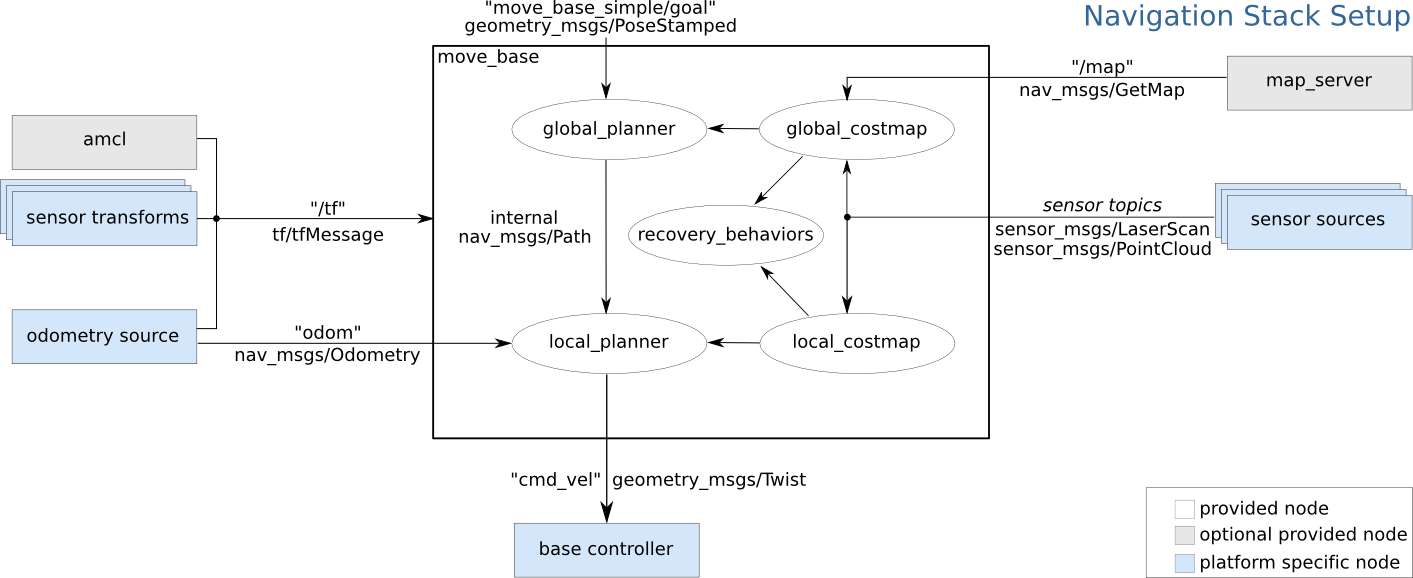
\includegraphics[width=\textwidth]{./figures/parts/01/chapters/03/sections/01/move_base.png}
  \caption{\small Εποπτική άποψη του λογισμικού αυτόνομης πλοήγησης
           \texttt{move\_base}. Πηγή: \url{http://wiki.ros.org/move\_base}}
  \label{fig:movebase}
\end{figure}

Το ROS έχει γίνει ευρέως δημοφιλές στην κοινότητα της ρομποτικής καθώς
προσφέρει μια πληθώρα δωρεάν πακέτων από ερευνητικές ομάδες όλου του κόσμου.
Προσφέρει δυνατότητες πλοήγησης με τη μορφή \textit{στοιβών}, δηλαδή
συλλογών πακέτων λογισμικού. Το πιο γνωστό και συχνά χρησιμοποιούμενο από αυτά
είναι το \texttt{\textbf{move\_base}}, το οποίο εσωτερικά χρησιμοποιεί έναν
αλγόριθμο κατασκευής μονοπατιών και έναν ελεγκτή κίνησης για να φέρει εις πέρας
το έργο της αυτόνομους πλοήγησης ρομπότ κινητής βάσης. Στην εσωτερική
ονοματολογία του ROS αυτά τα δύο συστατικά ονομάζονται αντίστοιχα
\textit{global planner} και \textit{local planner}. Το \texttt{move\_base}
παίρνει πληροφορίες από την οδομετρία, μετρήσεις από αισθητήρες, και μια
στάση-στόχο, και εξάγει ασφαλείς εντολές ταχύτητας προς είσοδο στους κινητήρες
κινητής βάσης.\footnote{\url{http://wiki.ros.org/navigation}} Ένα υψηλού
επιπέδου διάγραμμα αρχιτεκτονικής του απεικονίζεται στο σχήμα
\ref{fig:movebase}.

Κοιτώντας το \texttt{move\_base} ως ένα μαύρο κουτί, αυτό εξάγει ταχύτητες
κινητήρων, και προϋποθέτει την ύπαρξη των ακόλουθων εισόδων, είτε σε μορφή
μηνυμάτων ROS (δομημένα δεδομένα) ή μετασχηματισμών (σχέσεις μεταξύ συστημάτων
αναφοράς):

\begin{itemize}
  \item Την εκτιμώμενη στάση του ρομπότ με τη μορφή ενός μετασχηματισμού μεταξύ
        του οδομετρικού συστήματος αναφοράς του ρομπότ και του συστήματος
        αναφοράς του χάρτη, που παρέχεται εδώ από το
        \texttt{amcl}\footnote{\url{http://wiki.ros.org/amcl}} πακέτο ROS.
        AMCL σημαίνει Adaptive Monte Carlo Localisation \cite{amcl}
        και είναι επί του παρόντος ο de facto αλγόριθμος παρακολούθησης της
        στάσης ενός ρομπότ μέσα στον χώρο στο οικοσύστημα ROS
  \item Τους μετασχηματισμούς μεταξύ των συστημάτων αναφοράς
        των αισθητήρων και των τελικών στοιχείων (effectors) του ρομπότ
        χρησιμοποιώντας τον μηχανισμό μετασχηματισμού του ROS (\texttt{tf})
  \item Πληροφορίες οδομετρίας και (προαιρετικά) τον χάρτη του περιβάλλοντος
  \item Δεδομένα απόστασης είτε από έναν αισθητήρα αποστάσεων τύπου lidar, είτε
        από έναν αισθητήρα που μπορεί να εξάγει νέφη σημείων σε τρεις
        διαστάσεις, όπως μια κάμερα βάθους
\end{itemize}

Επιπλέον, το ROS προσφέρει μια αναπαράσταση του περιβάλλοντος που ονομάζεται
\textit{costmap}, που περιλαμβάνει πληροφορίες σχετικά με τη δυνατότητα
διέλευσης του ρομπότ μέσα στο περιβάλλον του και μέσα στον χάρτη αυτού, με βάση
το αποτύπωμα του ρομπότ και τα στατικά και δυναμικά εμπόδια (υποθέτοντας ότι
είναι πιο δαπανηρό να να κινηθεί κοντά σε εμπόδια). Όταν θεωρείται ως λευκό
κουτί, το \texttt{move\_base} περιλαμβάνει:

\begin{itemize}
  \item Έναν \textit{global costmap}, που αναπαριστά το κόστος διέλευσης πλησίον
        των στατικών εμποδίων του χάρτη
  \item Έναν \textit{local costmap} ο οποίος δημιουργείται και ανανεώνεται σε
        πραγματικό χρόνο στην άμεση γειτονιά του ρομπότ, και που βασίζεται στις
        μετρήσεις των εξωδεκτικών αισθητήρων προκειμένου να αντιμετώπισει τα
        στατικά και δυναμικά εμπόδια του πραγματικού περιβάλλοντός του
  \item Έναν \textit{global planner}, ο οποίος λαμβάνει ως είσοδο μία
        στάση-στόχο, και τον global costmap, και παράγει το γεωμετρικό μονοπάτι
        που ενώνει την αρχική στάση του ρομπότ με την επιθυμητή
  \item Έναν \textit{local planner}, ο οποίος δέχεται ως είσοδο το ως άνω
        μονοπάτι και τον local costmap και υπολογίζει εντολές ταχύτητας
  \item Μια ενότητα που ονομάζεται \texttt{recovery\_behaviours} που δέχεται και
        τους δύο χάρτες κόστους ως είσοδο, εντοπίζει πότε το ρομπότ δεν μπορεί
        να προχωρήσει με την επιθυμητή ταχύτητα, και εφαρμόζει προκαθορισμένα
        σύνολα κινήσεων, με στόχο την "απεγκλωβισμό" του ρομπότ. Αυτές οι
        ενέργειες ενεργοποιούνται κάθε φορά που (α) το ρομπότ γίνεται αντιληπτό
        ότι ταλαντώνεται, (β) ένα σχέδιο κίνησης δεν έχει ληφθεί για κάποιο
        χρονικό διάστημα, ή (γ) ο ελεγκτής κίνησης έχει αποτύχει να εξάγει
        έγκυρες εντολές ταχύτητας για ένα καθορισμένο χρονικό διάστημα.
        Συγκεκριμένα, το \texttt{move\_base} εφαρμόζει δύο είδη ανάκτησης του
        ελέγχου του ρομπότ: (α) μια περιστροφή $360$ μοιρών που στοχεύει στην
        εκκαθάριση του τοπικού χάρτη κόστους από τυχόν ψευδείς μετρήσεις
        (ψευδώς θετικά αντιληπτά εμπόδια) και (β) μια επαναφορά του χάρτη
        κόστους που καθαρίζει την στοίβα πλοήγησης επαναφέροντάς τον στον
        στατικό χάρτη έξω τα όρια μιας δεδομένης ακτίνας μακριά από το
        ρομπότ\footnote{\url{http://wiki.ros.org/clear\_costmap\_recovery}}.  Η
        τελευταία χρησιμοποιείται συνήθως πολλαπλές φορές και σε έναν ιεραρχικό
        τρόπο, ξεκινώντας από κάποια ακτίνα εντός του ημιπλάτους του τοπικού
        χάρτη κόστους και προχωρώντας πιο κοντά στο ίχνος του ρομπότ. Εάν το
        ρομπότ εξακολουθεί να θεωρείται παγιδευμένο μετά την εκτέλεση όλων των
        προκαθορισμένων συμπεριφορές αποκατάστασης η πλοήγηση διακόπτεται και
        το ρομπότ σταματά την κίνησή του, τουλάχιστον μέχρι να δοθεί ένας νέος
        στόχος.
\end{itemize}
